\chapter{Método}
\label{Metodo}
\indent

O Plano Semestral de Trabalho, como o nome sugere, é exigido dos docentes do \ac{IFG} semestralmente nos termos da Resolução nº 9 do \ac{IFG}~\citep{resolucao}.
Este capítulo descreve o trabalho efetuado para prover a solução proposta para a geração do Plano Semestral de Trabalho.

%visao geral
Inicialmente foi realizado um levantamento de requisitos funcionais com base na Resolução nº 9~\citep{resolucao} e em entrevista com o próprio orientador que é um usuário em potencial do sistema (\textit{stakeholder}).
Ao longo de \textit{Sprints} semanais, os avanços no desenvolvimento foram testados pelos \textit{stakeholders}.

%requisitos nao funcionais
Os requisitos não funcionais foram definidos a partir da proposta de melhoria na usabilidade do sistema. 
Como o sistema se propõem a ser mais completo que a planilha existente, centralizando o preenchimento dos dados e a geração do documento final, o formato Web responsivo se mostrou uma opção viável.

%prototipagem e RN
O próximo passo foi desenvolver telas de protótipos com base no levantamento inicial de requisitos, os quais são apresentados na Seção~\ref{RegrasDeNegocio}
A Seção~\nameref{Prototipos} apresenta os protótipos iniciais, acompanhados das regras de negócio que se aplicam a cada uma adas telas.

%desenvolvimento
Depois da validação dos protótipos com o \textit{stakeholder} e criação das regras de negócio com base no levantamento de requisitos, havia material suficiente para dar início a implementação do sistema.
O protótipo inicial e as regras de negócio foram ajustados de acordo com os retornos do \textit{stakeholder} ao final de cada \textit{Sprint}.
Neste capítulo as regas de negócio apresentadas são a versão final da documentação do sistema, enquanto os protótipos são apenas os iniciais.
No Capítulo~\nameref{Resultados} é apresentado o sistema em sua versão 1.0. 
A memória do desenvolvimento foi mantida num repositório no GitHub\footnote{https://github.com}.

%ferramentas
No desenvolvimento do \textit{back-end} foi utilizada a linguagem de programação \nameref{java} na versão 1.8 em conjunto do \nameref{spring} na versão 2.1.5, para a criação da lógica de negócio e construção da API~\nameref{rest} para fornecer os dados necessários para o \textit{front-end}. 
O~\nameref{mongo} na versão 4.0.9 foi utilizado para o armazenamento da base de dados.
No desenvolvimento do \textit{front-end} foi utilizado o \nameref{angular} na arquitetura e comunicação com o \textit{back-end} e em conjunto do \nameref{html} na versão 5, \nameref{css} e \nameref{bootstrap} na versão 4.3.4 foi construída a interface visual de interação do usuário.

%testes e implanatacao
Os testes e validação do sistema foram feitos pelo \textit{stakeholder} afim de verificar se os requisitos foram cumpridos e o objetivo final foi alcançado.
A implantação não ocorreu ainda e figurará como trabalhos futuros através do uso de um Docker container\footnote{http://dockerhub.com/}.

\newpage
\section{Protótipos}\label{Prototipos}
\subsection{Protótipo 01}\label{prototipo01}

A tela inicial (Protótipo 01) é mostrada na Figura~\ref{fig:prot01} e a descrição deste protótipo é mostrada na Tabela~\ref{tab:prot01}.

\begin{figure}[H]
    \centering
    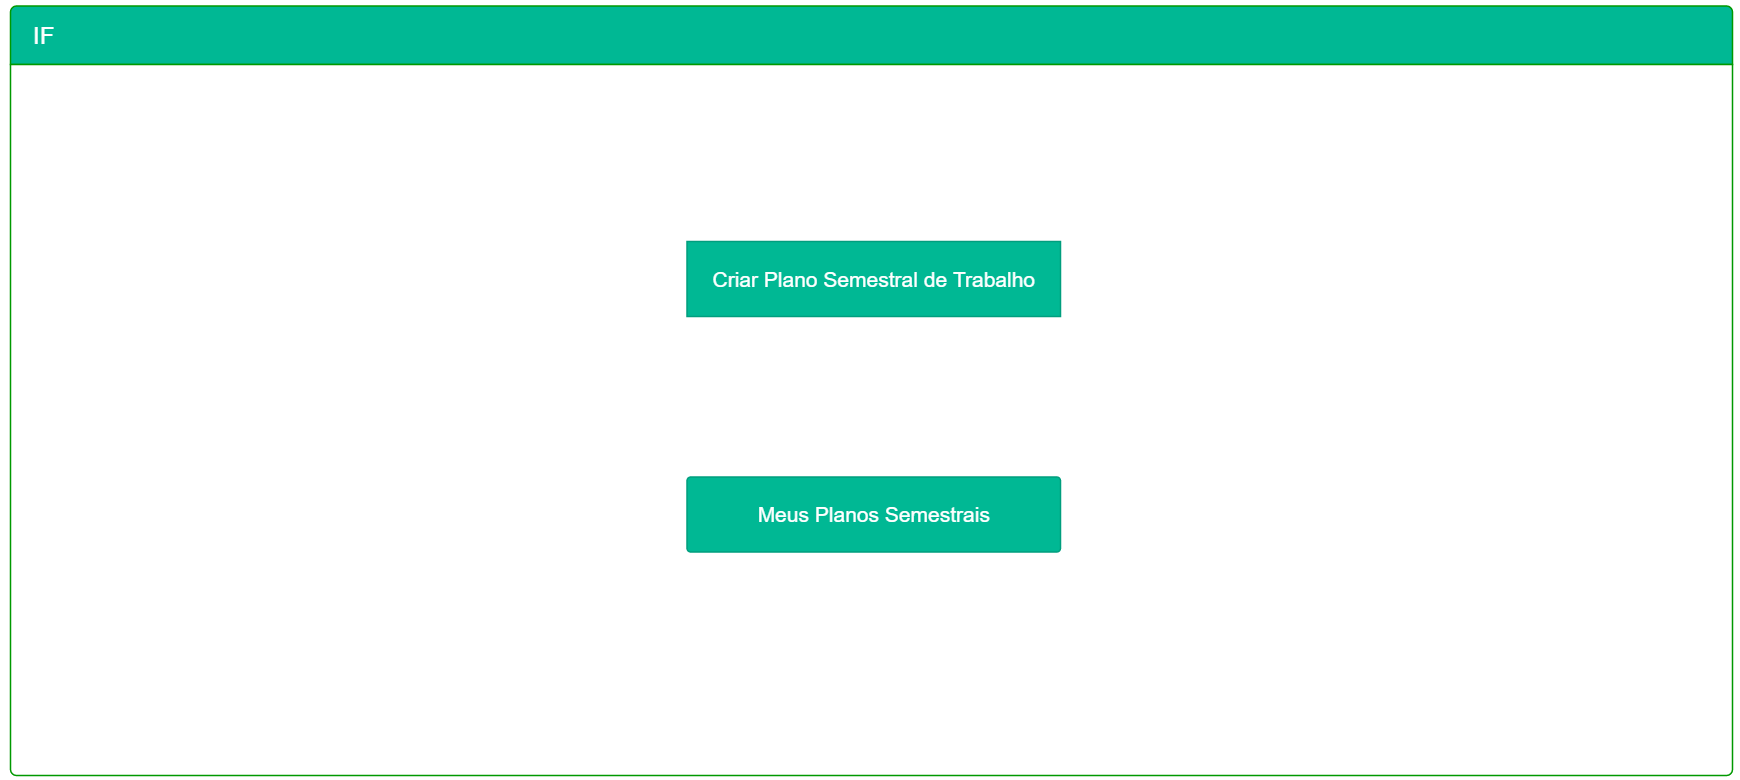
\includegraphics[width=0.95\textwidth]{img/1pagina_inicial.png}
    \caption[Protótipo 01: Tela inicial]{Protótipo 01: Tela inicial.}
    \label{fig:prot01}
\end{figure}

\begin{table}[H]
\centering
\caption[Tabela 01: Tabela descritiva do protótipo 01.]{Tabela 01: Tabela descritiva do protótipo 01.}
\label{tab:prot01}
\begin{tabular}{@{}lll@{}}
\toprule
Botões                &  Regras de Negócio                                \\ \midrule
Criar Plano Semestral de Trabalho      &     \nameref{rn016}              \\
Meus planos Semestrais                 &      \nameref{rn017}              \\ \bottomrule
\end{tabular}
\end{table}

\newpage
\subsection{Protótipo 02}\label{prototipo02}
A tela de identificação do professor (Protótipo 002) é mostrada na Figura~\ref{fig:prot02} e a descrição deste protótipo é mostrada na Tabela~\ref{tab:prot02}.


\begin{figure}[H]
    \centering
    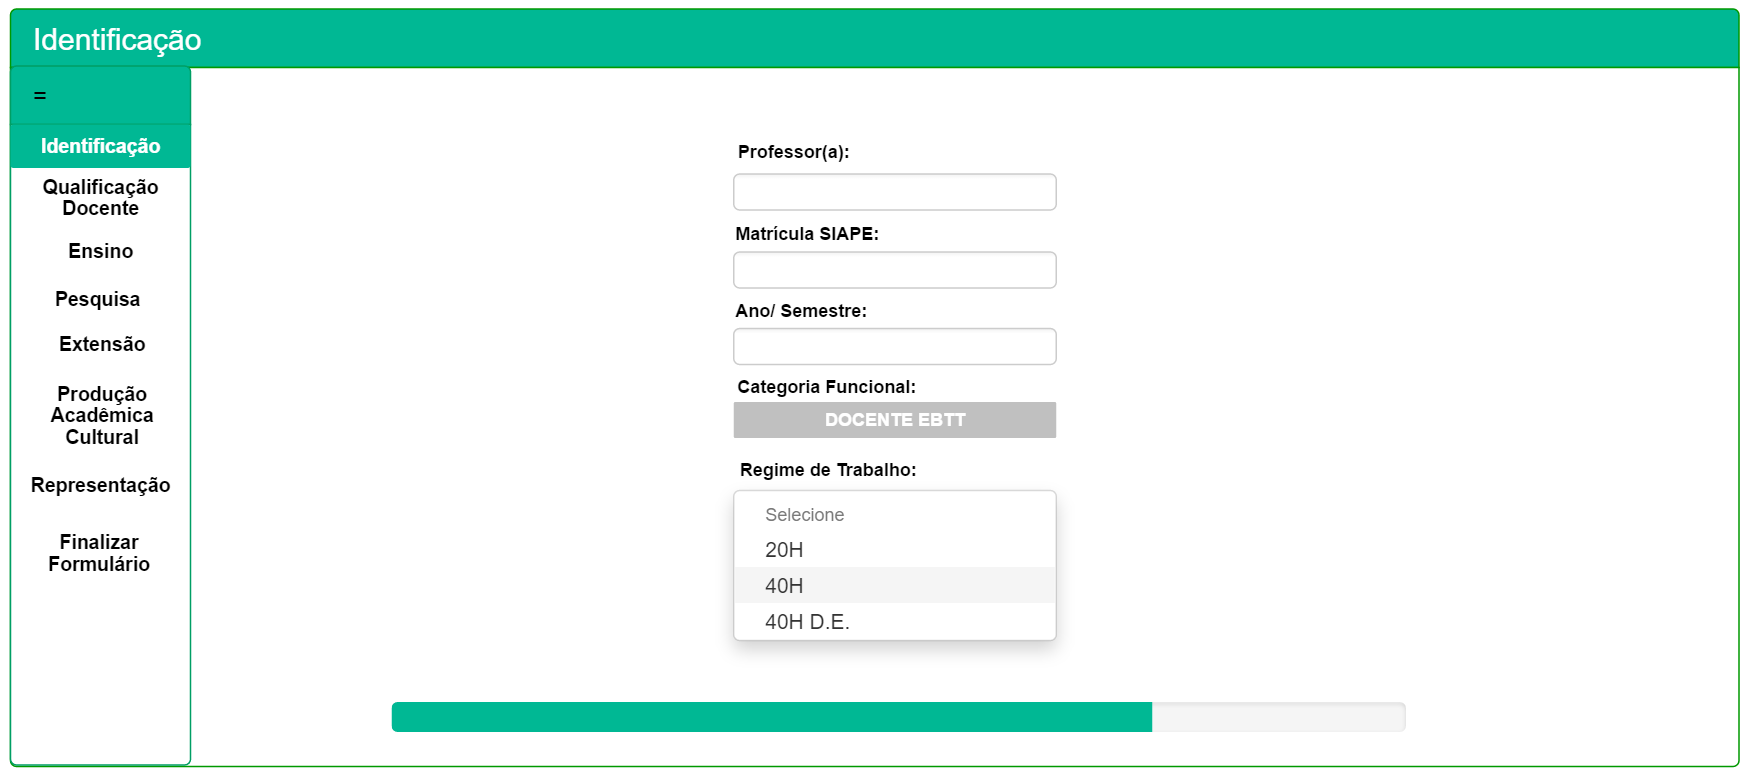
\includegraphics[width=0.95\textwidth]{img/2pagina_de_identificacao.png}
    \caption[Protótipo 02: Identificação]{Protótipo 02: Identificação.}
    \label{fig:prot02}
\end{figure}


\begin{table}[H]
\centering
\caption[Tabela 02: Tabela descritiva do protótipo 02.]{Tabela 02: Tabela descritiva do protótipo 02.}
\label{tab:prot02}
\begin{tabular}{@{}lll@{}}
\toprule
Campo               & Tipo     &  Regras de Negócio                     \\ \midrule
Professor(a)        & Texto    &    \nameref{rn002}, \nameref{rn004}    \\
Matrícula SIAPE     & Numérico &    \nameref{rn002}, \nameref{rn004}    \\
Ano/Semestre        & Texto    &    \nameref{rn002}, \nameref{rn004}    \\
Categoria Funcional & Texto    &    \nameref{rn003}, \nameref{rn004}    \\
Regime de Trabalho  & Seletor  &    \nameref{rn002}, \nameref{rn004}    \\ \bottomrule
\end{tabular}
\end{table}


\newpage
\subsection{Protótipo 03}\label{prototipo03}
A tela de qualificação do docente (Protótipo 03) é mostrada na Figura~\ref{fig:prot03} e a descrição deste protótipo é mostrada na Tabela~\ref{tab:prot03}.


\begin{figure}[H]
    \centering
    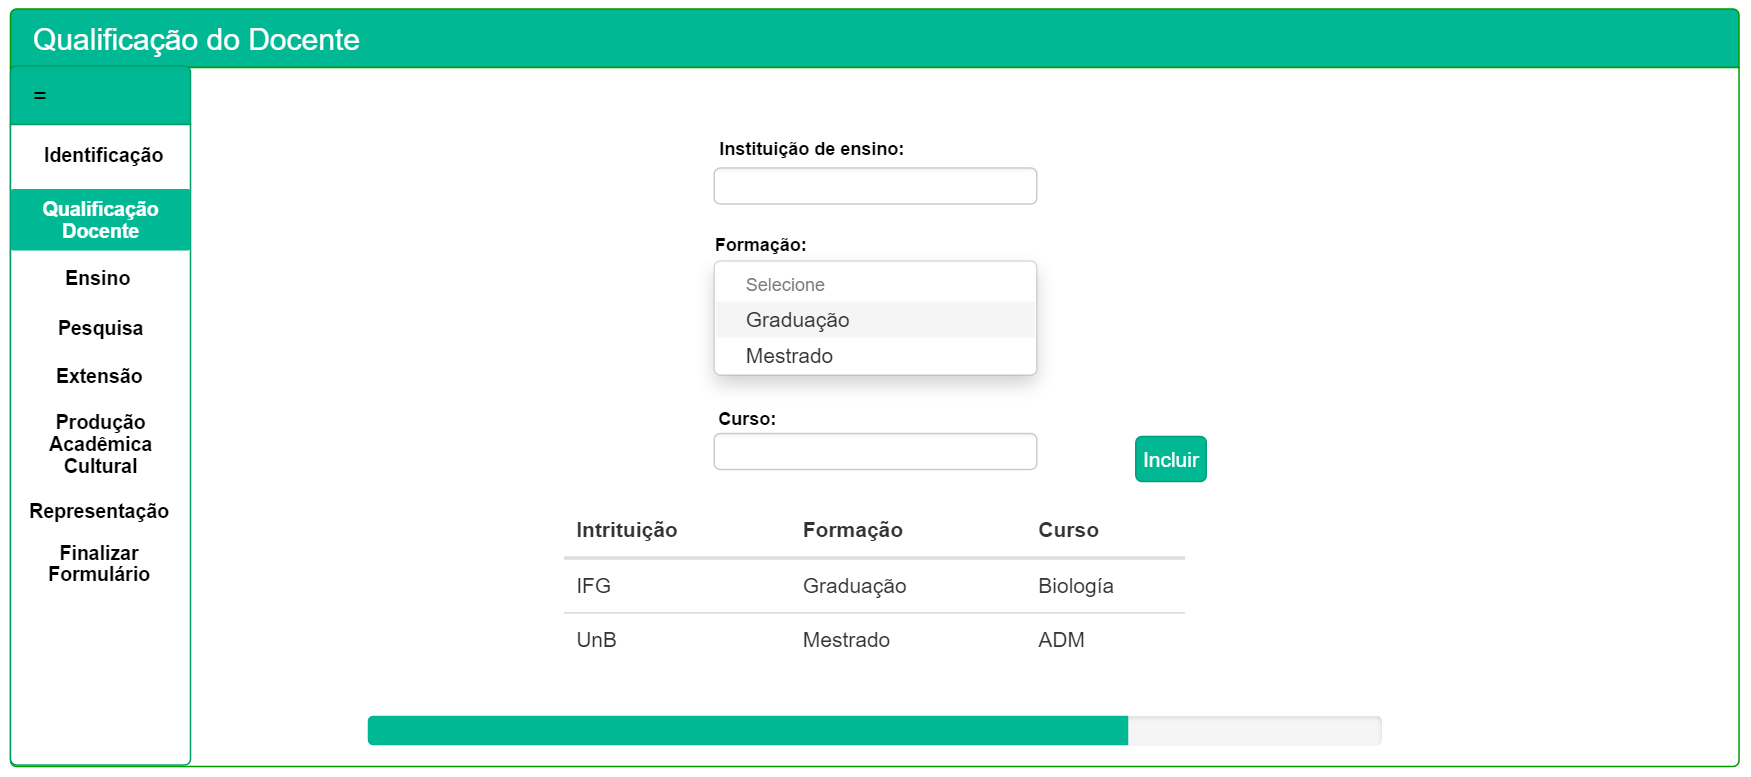
\includegraphics[width=0.95\textwidth]{img/3pagina_qualificacao_do_docente.png}
    \caption[Protótipo 03: Qualificação do Docente]{Protótipo 03: Qualificação do Docente.}
    \label{fig:prot03}
\end{figure}


\begin{table}[H]
\centering
\caption[Tabela 03: Tabela descritiva do protótipo 03.]{Tabela 03: Tabela descritiva do protótipo 03.}
\label{tab:prot03}
\begin{tabular}{@{}lll@{}}
\toprule
Campo                   & Tipo     &  Regras de Negócio                     \\ \midrule
Instituição de ensino   & Texto    &    \nameref{rn005}, \nameref{rn006}    \\
Formação                & Seletor  &    \nameref{rn005}, \nameref{rn006}    \\
Curso                   & Texto    &    \nameref{rn005}, \nameref{rn006}    \\ \bottomrule
\end{tabular}
\end{table}

\newpage
\subsection{Protótipo 04}\label{prototipo04}
A tela de atividades de ensino (Protótipo 04) é mostrada na Figura~\ref{fig:prot04} e a descrição deste protótipo é mostrada na Tabela~\ref{tab:prot04}.

\begin{figure}[H]
    \centering
    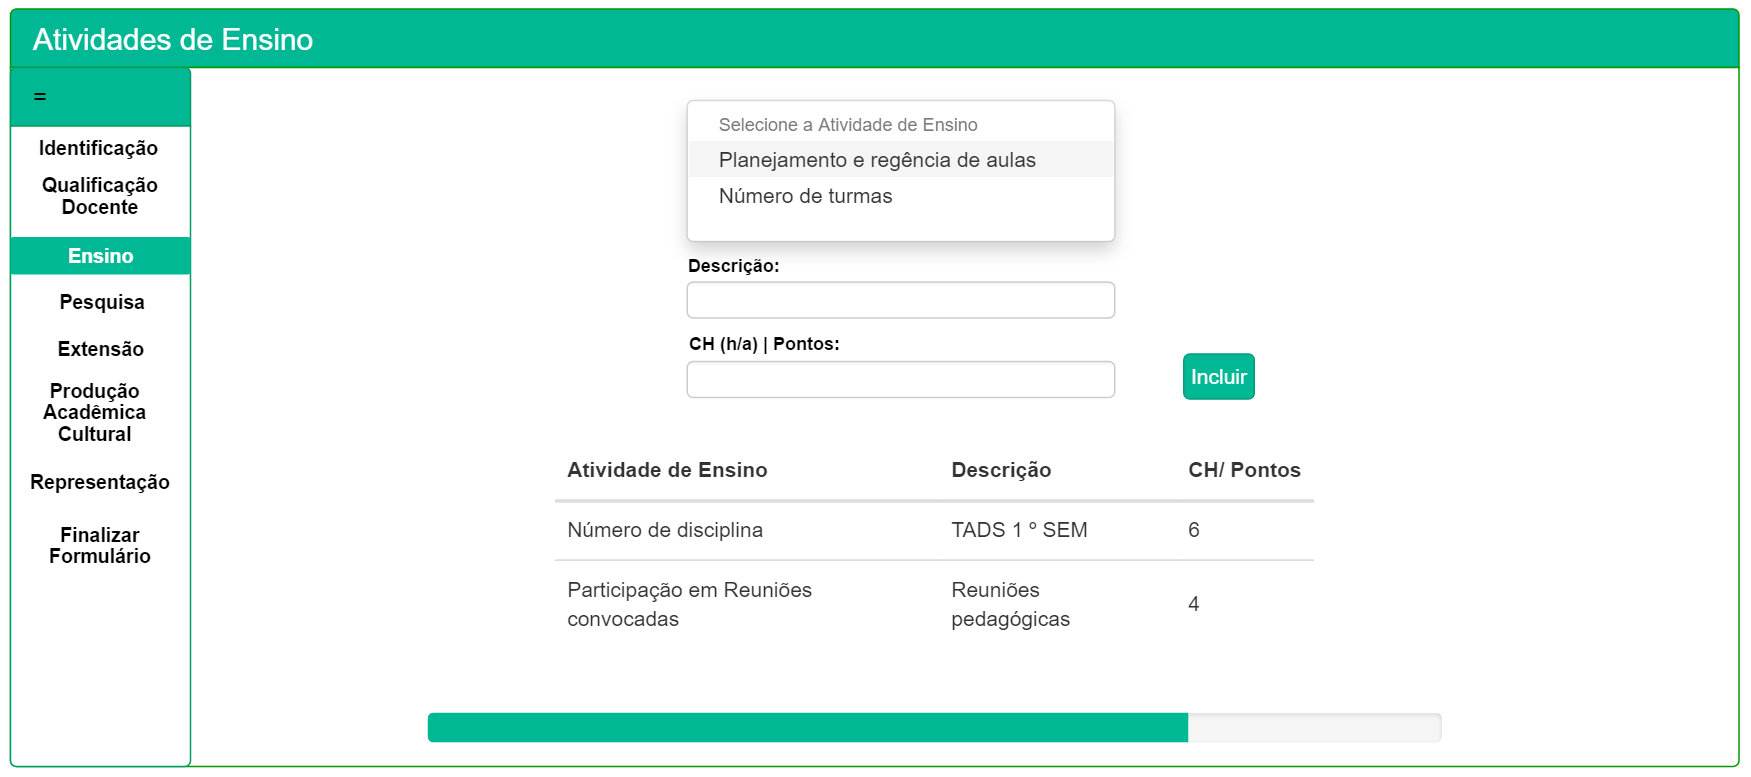
\includegraphics[width=0.95\textwidth]{img/4pagina_atividades_de_ensino.png}
    \caption[Protótipo 04: Atividade de Ensino]{Protótipo 04: Atividade de Ensino.}
    \label{fig:prot04}
\end{figure}

\begin{table}[H]
\centering
\caption[Tabela 04: Tabela descritiva do protótipo 04.]{Tabela 04: Tabela descritiva do protótipo 04.}
\label{tab:prot04}
\begin{tabular}{@{}lll@{}}
\toprule
Campo                           & Tipo     &  Regras de Negócio             \\ \midrule
Selecione a Atividade de Ensino & Seletor  &    \nameref{rn007}, \nameref{rn019}     \\
Descrição                       & Texto    &    \nameref{rn007}                 \\
CH(h/a)|Pontos:                 & Numérico &    \nameref{rn007}, \nameref{rn020}     \\ \bottomrule
\end{tabular}
\end{table}

\newpage
\subsection{Protótipo 05}\label{prototipo05}
A tela de atividades de pesquisa (Protótipo 05) é mostrada na Figura~\ref{fig:prot05} e a descrição deste protótipo é mostrada na Tabela~\ref{tab:prot05}.


\begin{figure}[H]
    \centering
    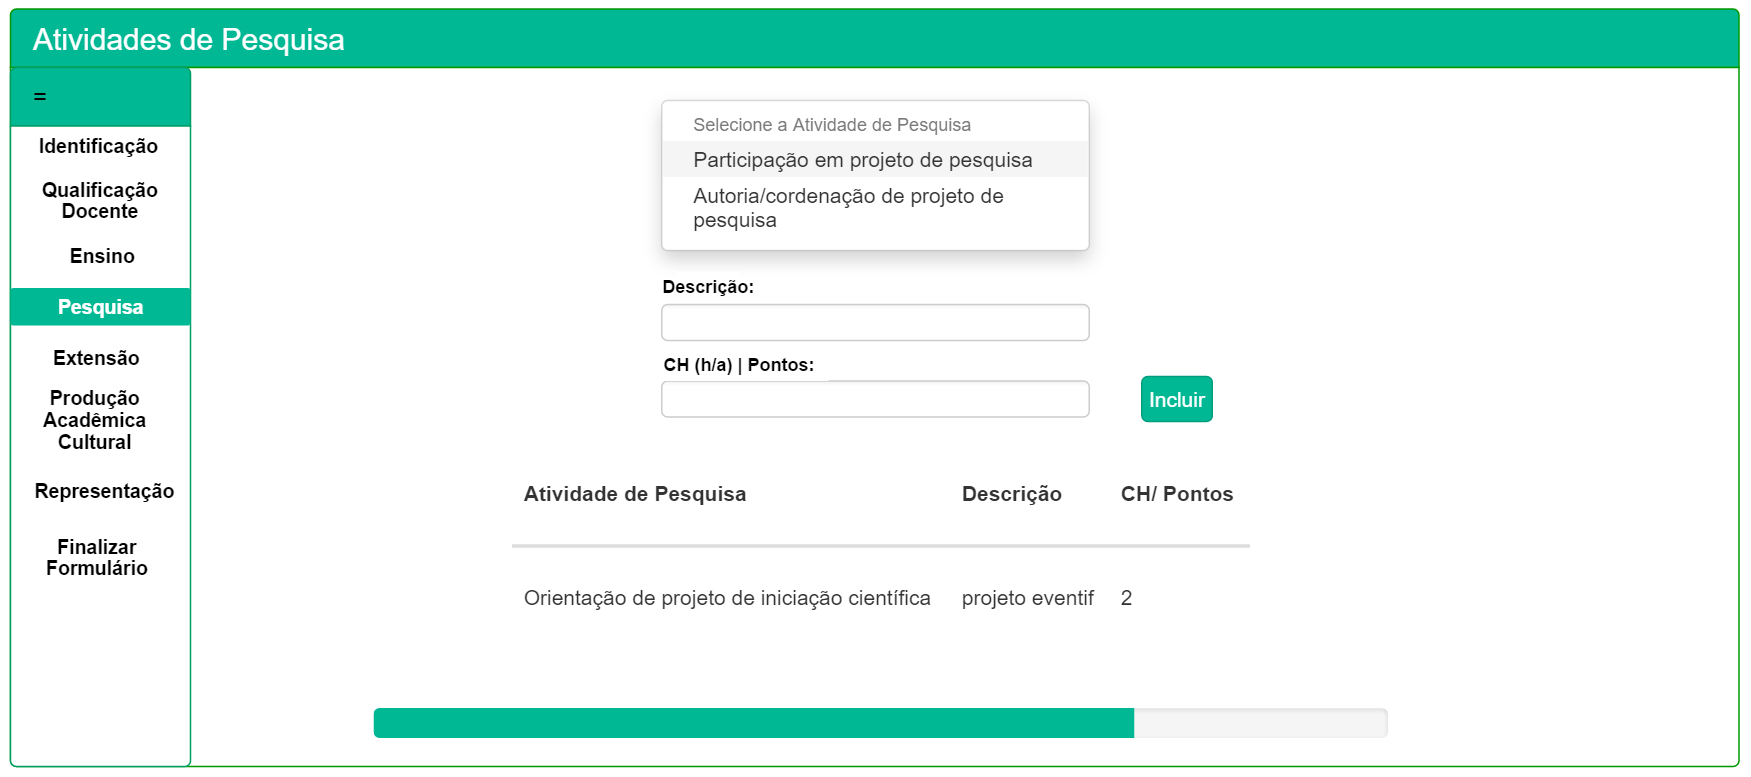
\includegraphics[width=0.95\textwidth]{img/5pagina_pesquisa.png}
    \caption[Protótipo 05: Atividade de Pesquisa]{Protótipo 05: Atividade de Pesquisa.}
    \label{fig:prot05}
\end{figure}


\begin{table}[H]
\centering
\caption[Tabela 05: Tabela descritiva do protótipo 05.]{Tabela 05: Tabela descritiva do protótipo 05.}
\label{tab:prot05}
\begin{tabular}{@{}lll@{}}
\toprule
Campo                             & Tipo     &  Regras de Negócio     \\ \midrule
Selecione a Atividade de Pesquisa & Seletor  &    \nameref{rn008}, \nameref{rn019}\\
Descrição                         & Texto    &    \nameref{rn008}                 \\
CH(h/a)|Pontos:                   & Numérico &    \nameref{rn008}, \nameref{rn020}\\ \bottomrule
\end{tabular}
\end{table}

\newpage
\subsection{Protótipo 06}\label{prototipo06}
A tela de atividades de extensão (Protótipo 06) é mostrada na Figura~\ref{fig:prot06} e a descrição deste protótipo é mostrada na Tabela~\ref{tab:prot06}.


\begin{figure}[H]
    \centering
    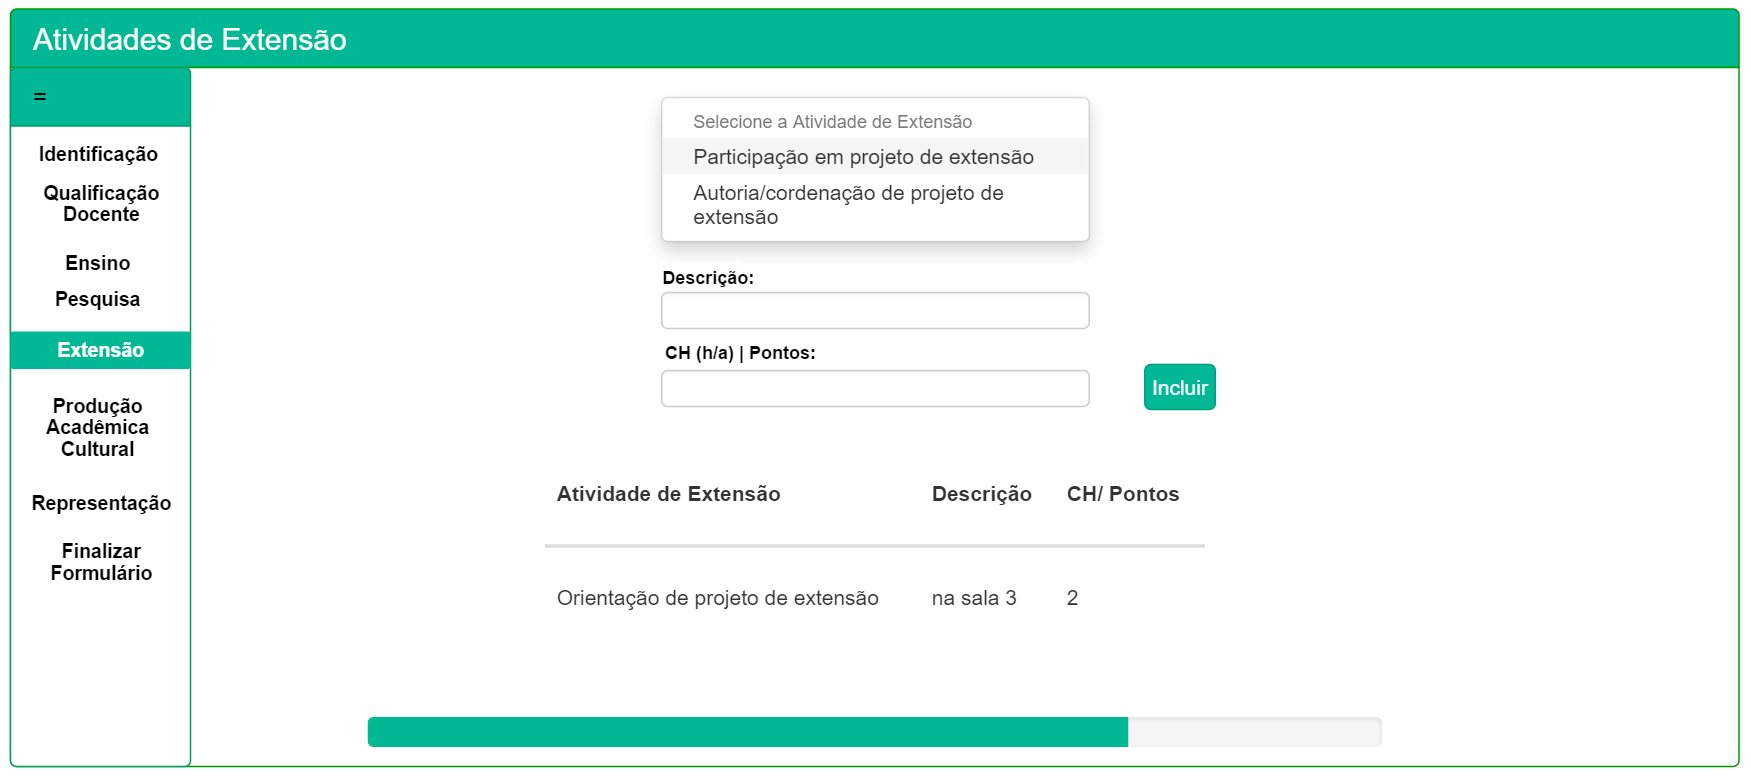
\includegraphics[width=0.95\textwidth]{img/6pagina_extensao.png}
    \caption[Protótipo 06: Atividade de Extensão]{Protótipo 06: Atividade de Extensão.}
    \label{fig:prot06}
\end{figure}


\begin{table}[H]
\centering
\caption[Tabela 06: Tabela descritiva do protótipo 06.]{Tabela 06: Tabela descritiva do protótipo 06.}
\label{tab:prot06}
\begin{tabular}{@{}lll@{}}
\toprule
Campo                             & Tipo     &  Regras de Negócio     \\ \midrule
Selecione a Atividade de Extensão & Seletor  &    \nameref{rn009}, \nameref{rn019}\\
Descrição                         & Texto    &    \nameref{rn009}                 \\
CH(h/a)|Pontos:                   & Numérico &    \nameref{rn009}, \nameref{rn020}\\ \bottomrule
\end{tabular}
\end{table}

\newpage
\subsection{Protótipo 07}\label{prototipo07}
A tela de atividades de produção acadêmica cultural (Protótipo 07) é mostrada na Figura~\ref{fig:prot07} e a descrição deste protótipo é mostrada na Tabela~\ref{tab:prot07}.


\begin{figure}[H]
    \centering
    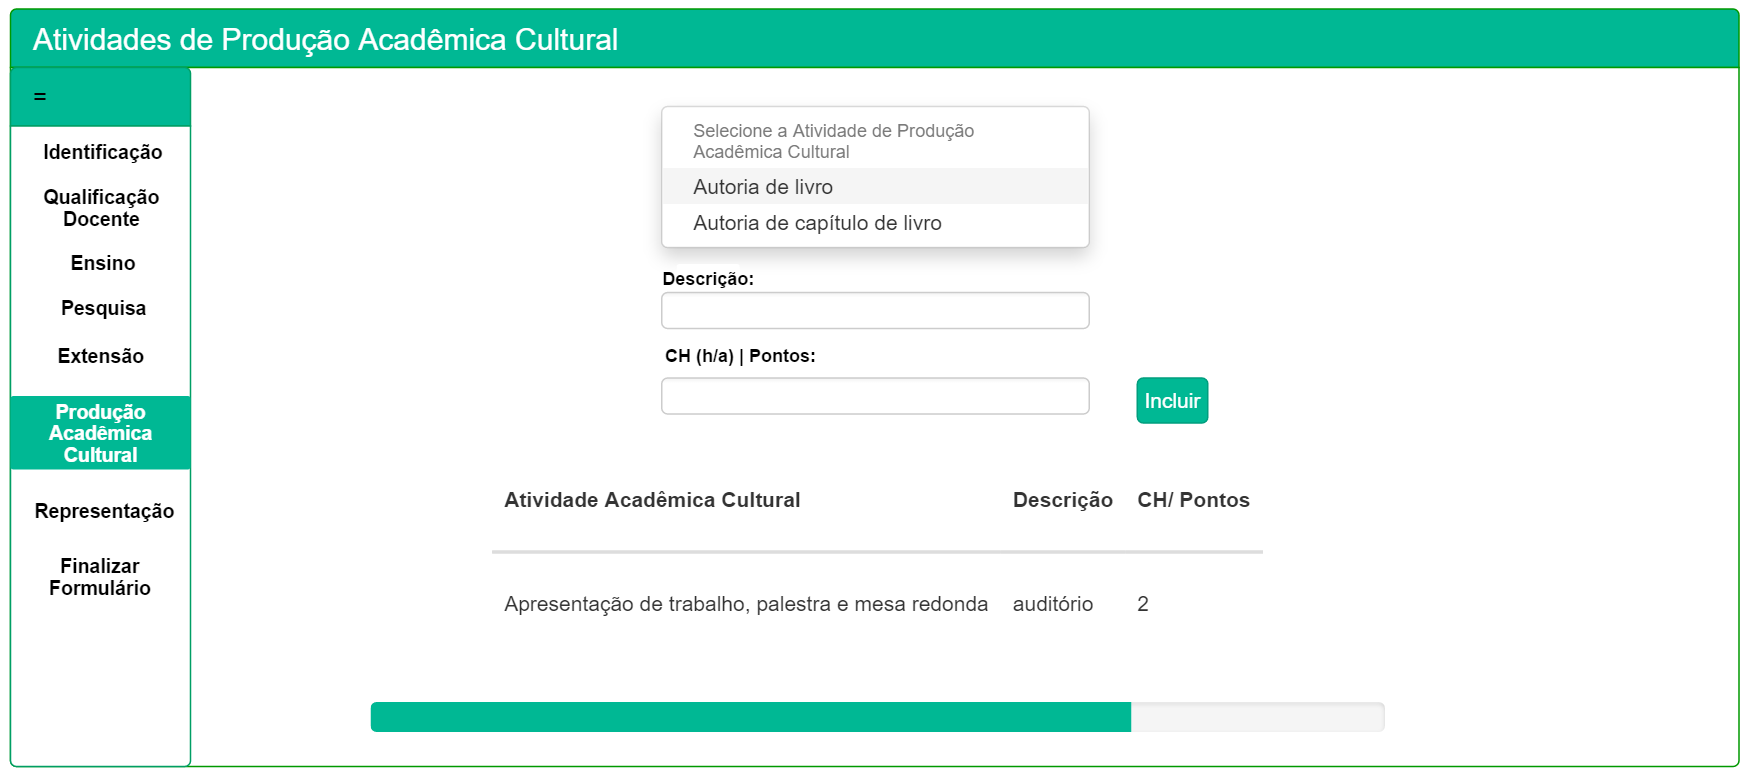
\includegraphics[width=0.95\textwidth]{img/7pagina_de_prod_academica.png}
    \caption[Protótipo 07: Atividade de Produção Acadêmica Cultural]{Protótipo 07: Atividade de Produção Acadêmica Cultural.}
    \label{fig:prot07}
\end{figure}


\begin{table}[H]
\centering
\caption[Tabela 07: Tabela descritiva do protótipo 07.]{Tabela 07: Tabela descritiva do protótipo 07.}
\label{tab:prot07}
\begin{tabular}{@{}lll@{}}
\toprule
Campo                                                & Tipo     &  Regras de Negócio     \\ \midrule
Selecione a Atividade de Produção Acadêmica Cultural & Seletor  &    \nameref{rn010}, \nameref{rn019}\\
Descrição                                            & Texto    &    \nameref{rn010}                 \\
CH(h/a)|Pontos:                                      & Numérico &    \nameref{rn010}, \nameref{rn020}\\ \bottomrule
\end{tabular}
\end{table}

\newpage
\subsection{Protótipo 08}\label{prototipo08}

A tela de atividades de representação (Protótipo 08) é mostrada na Figura~\ref{fig:prot08} e a descrição deste protótipo é mostrada na Tabela~\ref{tab:prot08}.

\begin{figure}[H]
    \centering
    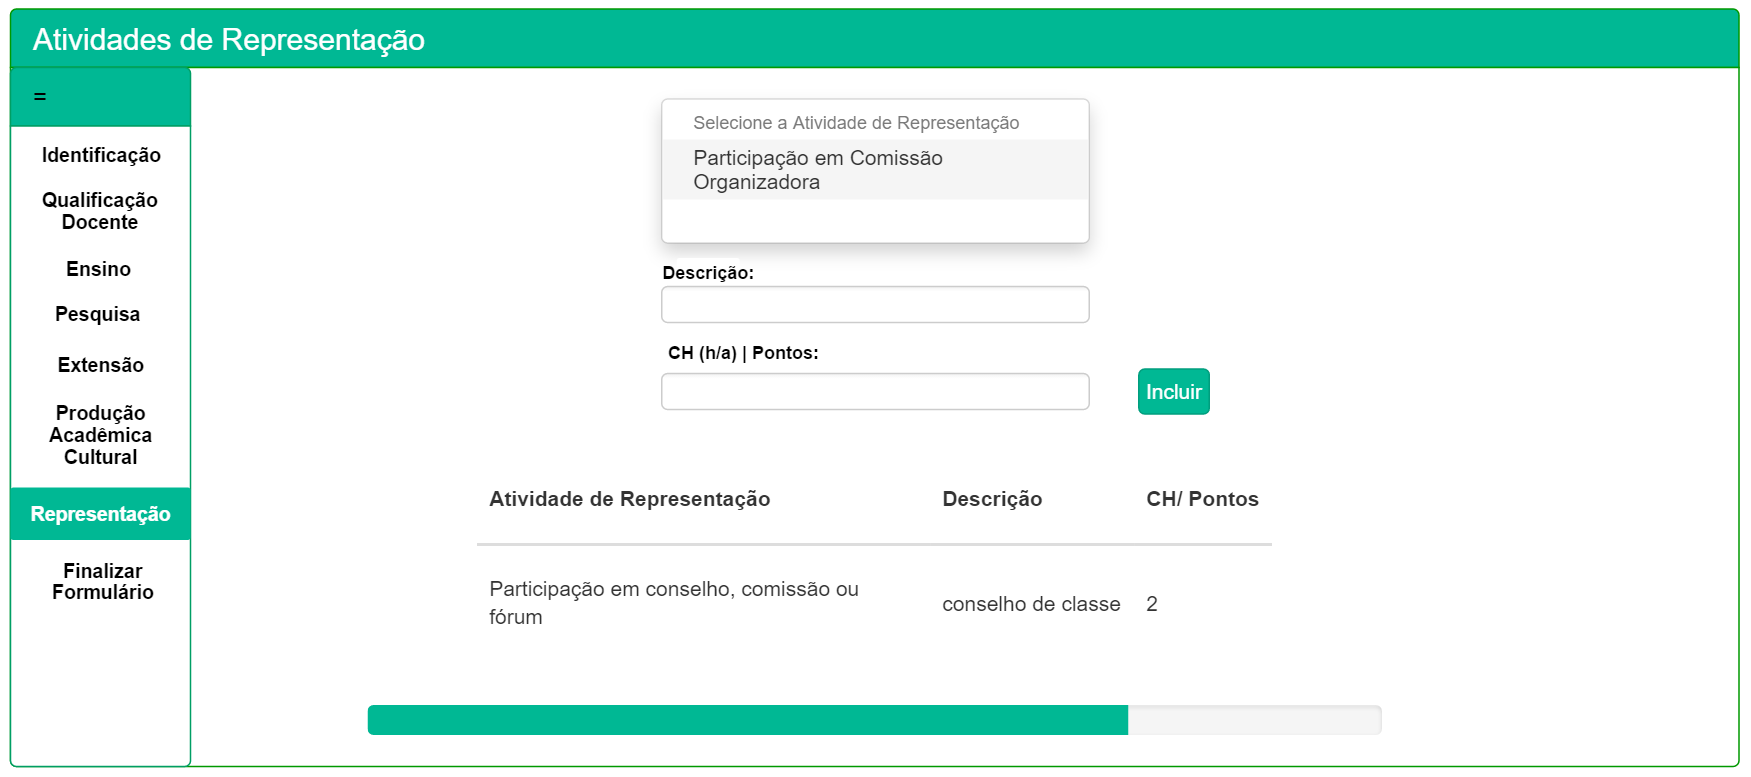
\includegraphics[width=0.95\textwidth]{img/8pagina_representacao.png}
    \caption[Protótipo 08: Atividade de Representação]{Protótipo 08: Atividade de Representação.}
    \label{fig:prot08}
\end{figure}


\begin{table}[H]
\centering
\caption[Tabela 08: Tabela descritiva do protótipo 08.]{Tabela 08: Tabela descritiva do protótipo 08.}
\label{tab:prot08}
\begin{tabular}{@{}lll@{}}
\toprule
Campo                                   & Tipo     &  Regras de Negócio     \\ \midrule
Selecione a Atividade de Representação  & Seletor  &    \nameref{rn011}, \nameref{rn019}\\
Descrição                               & Texto    &    \nameref{rn011}                 \\
CH(h/a)|Pontos:                         & Numérico &    \nameref{rn011}, \nameref{rn020}\\ \bottomrule
\end{tabular}
\end{table}

\newpage
\subsection{Protótipo 09}\label{prototipo09}
A tela de finalizar o formulário (Protótipo 09) é mostrada na Figura~\ref{fig:prot09} e a descrição deste protótipo é mostrada na Tabela~\ref{tab:prot09}.


\begin{figure}[H]
    \centering
    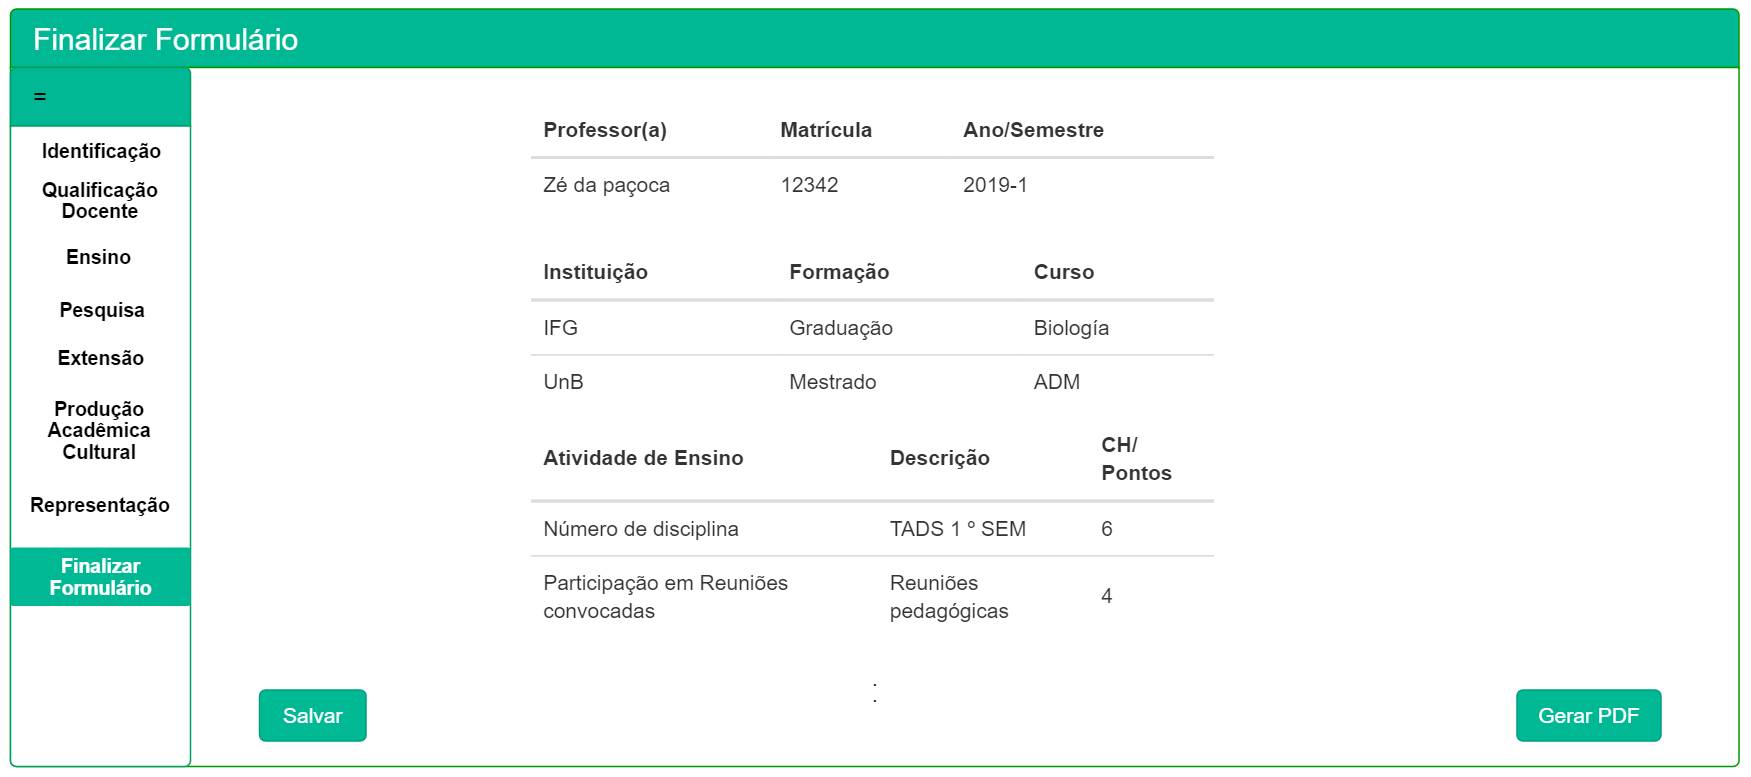
\includegraphics[width=0.95\textwidth]{img/9pagina_finalizar_formulario.png}
    \caption[Protótipo 09: Finalizar Formulário]{Protótipo 09: Finalizar Formulário.}
    \label{fig:prot09}
\end{figure}


\begin{table}[H]
\centering
\caption[Tabela 09: Tabela descritiva do protótipo 09.]{Tabela 09: Tabela descritiva do protótipo 09.}
\label{tab:prot09}
\begin{tabular}{@{}lll@{}}
\toprule
Botões      &  Regras de Negócio                                \\ \midrule
Salvar      &     \nameref{rn012}, \nameref{rn015}              \\
Gerar PDF   &     \nameref{rn012}, \nameref{rn014}              \\ \bottomrule
\end{tabular}
\end{table}



\newpage
\section{Regras de Negócio}\label{RegrasDeNegocio}

\subsection{RN001}\label{rn001}

O usuário deve ser um professor(a) do IFG.

\subsection{RN002}\label{rn002}

O usuário deve informar no menu ``Identificação'' os seguintes dados: Nome, matrícula SIAPE, ano/semestre, \textit{e-mail} e regime de trabalho.

\subsection{RN003}\label{rn003}

A informação sobre a categoria funcional do usuário deve ser incluída por padrão pelo sistema. Esse valor deve ser: DOCENTE EBTT.

\subsection{RN004}\label{rn004}

Todos os campos do menu ``Identificação'' são obrigatórios. 

\subsection{RN005}\label{rn005}

O usuário deve informar no menu ``Qualificação do Docente'' os seguintes dados: Instituição de ensino, formação e curso.

\subsection{RN006}\label{rn006}

Todos os campos do menu ``Qualificação do Docente'' são obrigatórios. 

\subsection{RN007}\label{rn007}

O usuário deve informar no menu ``Ensino'' os seguintes dados: A atividade de ensino, descrição e a carga horária ou pontuação. 

\subsection{RN008}\label{rn008}

O usuário deve informar no menu ``Pesquisa'' os seguintes dados: A atividade de pesquisa, descrição e a carga horária ou pontuação. 

\subsection{RN009}\label{rn009}

O usuário deve informar no menu ``Extensão'' os seguintes dados: A atividade de extensão, descrição e a carga horária ou pontuação.

\subsection{RN010}\label{rn010}

O usuário deve informar no menu ``Produção Acadêmica Cultural'' os seguintes dados: A atividade de produção acadêmica cultural, descrição e a carga horária ou pontuação.

\subsection{RN011}\label{rn011}

O usuário deve informar no menu ``Atividade de Qualificação'' os seguintes dados: A atividade de qualificação, descrição e a carga horária ou pontuação.

\subsection{RN012}\label{rn012}

O usuário deve informar no menu ``Representação'' os seguintes dados: A atividade de representação, descrição e a carga horária ou pontuação.

\subsection{RN013}\label{rn013}

O usuário deve verificar as informações de seu formulário no menu ``Finalizar Formulário''.

\subsection{RN014}\label{rn014}

O usuário deve ter uma somatória de pontos correspondente a carga horária do regime de trabalho preenchida na regra de negócio [\nameref{rn002}]

\subsection{RN015}\label{rn015}

No menu ``Finalizar Formulário'' o usuário deve clicar no botão ``Gerar PDF'' para gerar o \ac{PDF} do formulário plano semestral de trabalho.

\subsection{RN016}\label{rn016}

No menu ``Finalizar Formulário'' o usuário deve clicar no botão "Salvar" para salvar o formulário plano semestral de trabalho.

\subsection{RN017}\label{rn017}

Na página inicial o usuário deve clicar no botão ``Criar Plano Semestral de Trabalho'' para iniciar o formulário.

\subsection{RN018}\label{rn018}

Na página inicial o usuário deve clicar no botão ``Meus Planos Semestrais'' para recuperar um formulário já existente.

\subsection{RN019}\label{rn019}

A atividade de uma categoria só pode ser selecionada uma vez, então o usuário deve preencher  na descrição todo o conteúdo relacionada com aquela determinada atividade, e no campo de carga horária ou pontuação preencher com o valor total destinado para a atividade em questão.

\subsection{RN020}\label{rn020}

O campo de carga horária ou pontuação tem valor máximo limitado de acordo com a Resolução 9~\citep{resolucao}.

\subsection{RN021}\label{rn021}

A tabela com a listagem de todas as atividades, pontuação e somatório encontra se na página de finalização do formulário.

